\section{Evaluation}
\label{sec:eval}

In this section we evaluate the framework of
wikification via link co-occurrence.
We first explain how we prepare Wikipedia corpus samples and the test data.
Then we discuss four experiments. The first experiment shows
the effects of using corpora of different sizes; the second one evaluates
the iterative algorithm which generates the co-occurrence
matrix; the third one compares the end-to-end wikification results from
our framework with the baseline as well as four state-of-the-art methods;
while the last experiment measures the time performance of our system.
The Wikipedia corpus we use was a complete dump \cite{wikipedia} (27GB)
published in May 2011 which contains 8.56 million surface forms and
3.28 million unique concepts (senses). All experiments in this section
are conducted on a 64-bit workstation with 3.10 GHz quad-core Intel CPU
and 16 GB memory running Windows Server 2008.
%Before we present the experimental results, let's first
%look at how we prepare the corpus and our test data.


\subsection{Data Preparation}
\label{sec:testdata}
One of the important points to show in the evaluation is that
our framework doesn't require all of the Wikipedia articles to be
effective. But instead, samples of highly popular and information-rich
articles are enough to provide the co-occurrences we need for wikification.
Completely random samples don't guarantee information richness.
Our approach is to first collect a set of information-rich articles,
then apply random sampling on the set.
We obtain the set of information-rich articles by taking the top $3k$ articles
ordered by \emph{PageRank}\cite{Brin1998} within the Wikipedia network.
\emph{PageRank} ranks documents by their popularity.
We argue that articles which are referenced by many others are supposed
to have richer content.

To compute PageRank on the Wikipedia network,
each Wikipedia article is treated as a web page, and links to the peers
are treated as hyperlinks in web pages.
As a bias towards longer articles, we set the initial \emph{PageRank}
to be proportional to the article length. Finally from the $3k$ informative articles, we randomly pick $k$ articles as
our sample corpus.
\cut{In the following experiments, we use
size different sample corpora where $k$ is
5,000, 10,000, 15,000, 20,000, 35,000 and 50,000.
$k = 10,000$ is our default sample size.}

Next we describe our test data sets.
Though there has been previous work on wikification,
no standard test data sets are available yet.
Bartunov et al.\cite{bartunov2011wikifyme} ran a project called
``WikifyMe" to create a standard test data for wikification.
Unfortunately, the web site doesn't provide sufficient data for our
test purposes.
In our evaluation, we use three test data sets.
The first two are publicly available data sets for wikification,
reported by Dai et al.\cite{daientity}.
They are created by Cucerzan\cite{cucerzan2007large} and
Kulkarni et al.\cite{kulkarni2009collective}, respectively.
Cucerzan's test data comes from
Wikipedia articles and news articles.
Because Wikipedia articles may have been modified
since Cucerzan finished his experiment, we only use the news articles.
Kulkarni's data set is complete with test corpus and labeled ground
truth.  The third test set is our own creation which is extracted from
25 articles of New York Times and China Daily covering five topics:
world, business, sports, entertainment and technology.
We parsed these paragraphs into unlinked terms and then
manually linked these terms to the appropriate Wikipedia articles
as the ground truth labels.

In the rest of this section, the three test sets are referred to as
Cucerzan's, Kulkarni's and Cai's, respectively. Examples from each of the three
test set (along with our wikification results) are shown in
\figref{fig:allthree}. The phrases disambiguated
are marked with underlines, with the disambiguated senses surrounded
by square brackets.

%The characteristics
%of the three data sets are listed in Table \ref{tab:char}.
%
%\begin{table}[th]
%\centering
%\begin{tabular}{|c|c|c|c|}
%\hline
%\multirow{2}*{Data} & Avg \# of & Avg \# of & \multirow{2}*{Topic} \\
%& Sentences & Words & \\
%\hline \hline
%\multirow{2}*{Cucerzan's} & \multirow{2}*{30.08} & \multirow{2}*{441.96} & World, Business, Life \\
%& & & Entertainment, Technology \\
%\hline
%\multirow{2}*{Kulkarni's} & \multirow{2}*{38.40} & \multirow{2}*{614.10} & World, Business, Life\\
%& & & Entertainment, Sports \\
%\hline
%\multirow{2}*{Cai's} & \multirow{2}*{5.25} & \multirow{2}*{87.7} & World, Business, Sports \\
%& & & Entertainment, Technology \\
%\hline
%\end{tabular}
%\caption{Average \# of Sentences and Words per Article and Topic}
%\label{tab:char}
%\end{table}

\begin{figure}
\centering
\fbox{
\begin{minipage}{\columnwidth}
{\scriptsize \tt
{\renewcommand\baselinestretch{1.0}\selectfont
\uline{Home Depot}[{The Home Depot}] CEO \uline{Nardelli}[{Robert Nardelli}] quits.\uline{Home}[{The Home Depot}] - improvement retailer's chief executive had been criticized over pay.ATLANTA - \uline{Bob Nardelli}[{Robert Nardelli}] said he had no intention of stepping down. ... (omitted)''
\par}
}
\end{minipage}
}
%\vspace*{2ex}
\fbox{
\begin{minipage}{\columnwidth}
{\scriptsize \tt
{\renewcommand\baselinestretch{1.0}\selectfont
On the Trail \uline{Nancy Pelosi}[{Nancy Pelosi}]: End the war for our kids' sake In this essay, the \uline{Speaker of the House}[{Speaker (politics)}] and mother of five calls for \uline{peace}[{Peace}] Mark Wilson / \uline{Getty Images}[{Getty Images}] file ... (omitted)''
\par}
}
\end{minipage}
}
%\vspace*{2ex}
\fbox{
\begin{minipage}{\columnwidth}
{\scriptsize \tt
{\renewcommand\baselinestretch{1.0}\selectfont
\uline{US Navy}[{United States Navy}]''s Operation Chief \uline{Jonathan Greenert}[{Jonathan W. Greenert}] on \uline{Wednesday}[{Wednesday}] said the \uline{Iranian Navy}[{Islamic Republic of Iran Navy}] has been "relatively quiet" in their dealing with \uline{US}[{United States}] ... (omitted)''
\par}
}
\end{minipage}
}
\caption{Snippets from The Three Test Data Set}
\label{fig:allthree}
\end{figure}

%\begin{figure}
%\centering
%\fbox{
%\begin{minipage}{\columnwidth}
%{\scriptsize \tt
%{\renewcommand\baselinestretch{1.0}\selectfont
%UNITED NATIONS - UN spokesman Martin Nesirky on Thursday called the recent attacks on a Syrian Television station ``regrettable and unacceptable.'' ``It's regrettable by any standards,''  Nesirky said at a daily news briefing here. ``Any violence that is happening in Syria at the moment should be ... (omitted)''
%\par}
%}
%\end{minipage}
%}
%\vspace*{2ex}
%\fbox{
%\begin{minipage}{\columnwidth}
%{\scriptsize \tt
%{\renewcommand\baselinestretch{1.0}\selectfont
%Asia's first Grand Slam champion Li Na has served up a volley of controversy on the Internet after complaining about playing doubles at the upcoming London Olympics. ``What's the point for me of playing the doubles? I have never played doubles since 2007 at the Australian Open. Why do they want me to play?''... (omitted)
%\par}
%}
%\end{minipage}
%}
%\caption{Two Snippets from Cai's Test Data Set}
%\label{fig:cai}
%\end{figure}

\subsection{Effects of Wikipedia Corpus Sizes}
In the first part of the evaluation, we would like to check the effect of
using different corpus size.
We run our experiment on five different samples.
\figref{fig:m_final} and \figref{fig:l_final} show the final number of pairs of
co-occurring concepts and linked terms after iteration on different
samples. We can see that both numbers are sub-linear to the corpus sizes,
indicating that increasing the sample size which increases the cost in
time and space doesn't give us proportional gain.
Our hypothesis is that, with a proper sampling strategy,
we can obtain sufficient knowledge in a small corpus.
To this end, we introduce {\em matrix coverage} as a measure to evaluate the
quality of sampling. Matrix coverage measures the number of concepts
appearing in the matrix. It's important because we can possibly
disambiguate a term into a concept only if the concept exists in our matrix.
Considering the fact that
different concepts differ in their popularity and importance,
we also calculate a weighted matrix coverage, i.e.,
we multiply the \emph{PageRank} score by the frequency of a concept.
\figref{fig:rows} and \figref{fig:scores} show the two versions of
matrix coverage. The values are sub-linear to sample sizes,
which supports our hypothesis.

\begin{figure}[th]
\begin{subfigure}[t]{0.49\columnwidth}
\centering
\epsfig{file=m_final.eps,width=1.05\columnwidth}
\caption{Final Matrix Size on Different Corpus Sizes}
\label{fig:m_final}
\end{subfigure}
\hfill
\begin{subfigure}[t]{0.49\columnwidth}
\centering
\epsfig{file=l_final.eps,width=1.05\columnwidth}
\caption{Final Number of Linked Terms on Different Corpus Sizes}
\label{fig:l_final}
\end{subfigure}
\caption{Final Matrix Size and Number of Linked Terms}
\end{figure}

\begin{figure}[th]
\begin{subfigure}[t]{0.49\columnwidth}
\centering
\epsfig{file=figure/rowsOnSamples.eps,width=1.05\columnwidth}
\caption{Concepts Covered in the Matrix on Different Corpus Sizes}
\label{fig:rows}
\end{subfigure}
\hfill
\begin{subfigure}[t]{0.49\columnwidth}
\centering
\epsfig{file=figure/weightedRowsOnSamples.eps,width=1.05\columnwidth}
\caption{Score of Covered Concepts on Different Corpus Sizes}
\label{fig:scores}
\end{subfigure}
\caption{Final Matrix Coverage}
\end{figure}

To get a straightforward view of the effect on wikification using
different corpus sizes, we conduct the next experiment. We take the
final matrix produced by different corpus size with $W_c = 15$ and
$\tau = 0.5$ to wikify
the three test data set. \figref{fig:result} shows the average
precision, recall and F1-measure of our wikification method on them.
%Wikification method achieves both high precision and high recall.
Result in different corpus sizes are similar to each other, indicating
that a small number of popular articles is good enough to %all you need to
bootstrap the matrix generation process, leading to a good wikification result.

\subsection{Iteration Results}
In the second part of the evaluation, we verify the correctness of the new links
added during the iterative enrichment algorithm.
The accuracy of the additional links is important because it affects the
distribution of the final matrix, thus affects the end-to-end wikification result.
%To see the quality of adding link in our iterative algorithm, both on Wikipedia
%articles and plain text, we design the following experiment.
We sample 20,000 articles from Wikipedia corpus and run our iterative process
to adding links to Wikipedia articles. When the iteration completes,
%and randomly pick 10000 articles
%from these 20000 articles. Links in these picked articles are removed to turn
%them into plain texts. For the group of 20000 articles, we apply the original
%iterative method on them. For the group of picked 10000 link-removed articles,
%we first build the initial co-occurrence matrix using the left 10000 articles,
%then apply the plain-text-version iterative method on them.
we manually check whether the added links are correct or not. The number of
added links and the accuracy in each iteration is shown in \figref{fig:2wlink}.
We sample 100 articles from those 20,000 articles. For each article, we pick
the first 50 added links in each iteration to form the data set,
forming about 5,000 links to be examined in each iteration.
From \figref{fig:2wlink} we can see that, our iterative process
significantly increases the links in Wikipedia corpus while the accuracy
in each iteration decreases slightly but stabilizes above 0.9.

\begin{figure}[th]
\centering
%\begin{subfigure}[t]{0.8\columnwidth}
%\centering
\epsfig{file=20000_link_accuracy.eps,width=0.7\columnwidth}
\caption{Number and Accuracy of New Links in Wikipedia}
\label{fig:2wlink}
%\end{subfigure}
%\begin{subfigure}[t]{0.8\columnwidth}
%\centering
%\epsfig{file=10000+10000_link_accuracy.eps,width=\columnwidth}
%\caption{Accuracy of Linking on Plain Text}
%\label{fig:1wpluslink}
%\end{subfigure}
%\caption{Accuracy of Linking}
\end{figure}

%During the iteration process,
%we output some information to a log file containing the number of linked term and co-occurrence
%matrix size (the number of pairs of two co-occurring concepts) after each iteration. So
%it's easy for us to test the quantity of our iterative method. \figref{fig:ms_sample} to \figref{fig:ln_window}
%show the size of the
%co-occurrence matrix and the number of linked terms in each iteration for different Wikipedia
%corpus sample size and different window size. We can see that the approach
%can significantly increase the number of linked terms.
%As a result, the size of the co-occurrence matrix is also increased
%tremendously. Also, our iterative method converges
%very fast. Both the matrix size and the number of linked term
%increase with the sample size. But \figref{fig:m_final} and
%\figref{fig:l_final} show that the relations are {\em sub-linear}.
%\figref{fig:ln_window} also shows that larger window sizes don't provide the
%bang with the buck, as it costs exponentially more to compute but produces
%only a few more links.

%\begin{figure*}
%\centering
%\begin{subfigure}[t]{0.8\columnwidth}
%\centering
%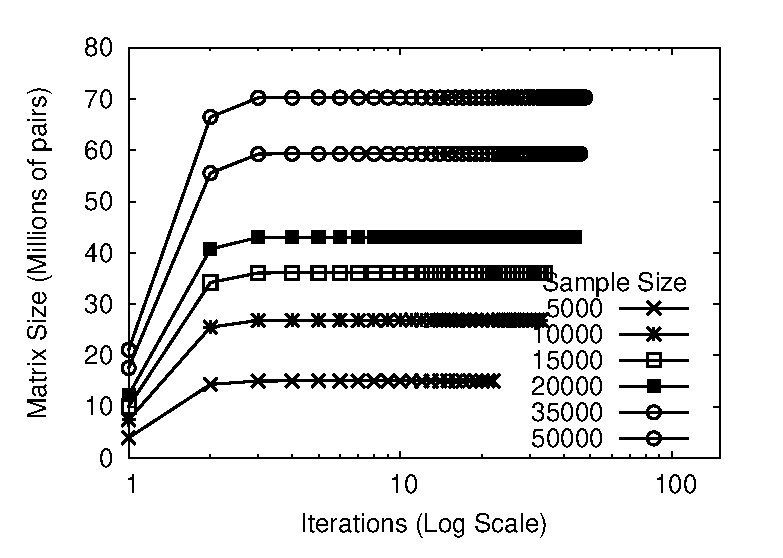
\epsfig{file=ms_sample.eps,width=\columnwidth}
%\caption{Matrix Sizes vs. Sample Sizes}
%\label{fig:ms_sample}
%\end{subfigure}
%\begin{subfigure}[t]{0.8\columnwidth}
%\centering
%\epsfig{file=ms_window.eps,width=\columnwidth}
%\caption{Matrix Sizes vs. Window Sizes}
%\label{fig:ms_window}
%\end{subfigure}
%\begin{subfigure}[t]{0.8\columnwidth}
%\centering
%\epsfig{file=ln_sample.eps,width=\columnwidth}
%\caption{\# of Links vs. Sample Sizes}
%\label{fig:ln_sample}
%\end{subfigure}
%\begin{subfigure}[t]{0.8\columnwidth}
%\centering
%\epsfig{file=ln_window.eps,width=\columnwidth}
%\caption{\# of Links vs. Window Sizes}
%\label{fig:ln_window}
%\end{subfigure}
%\caption{Behavier of Iterative Algorithm}
%\end{figure*}

Next is to test the effectiveness of our iterative process in
improving the end-to-end wikification result.
%To see the difference in the quality of the co-occurrence matrix {\em before}
%and {\em after} the iterations,
We use the original matrix and
final matrix to wikify the text in the three test data sets.
Sample size here is 10,000.
%and co-occurrence window size $W_c$ is set to be 15.
Table \ref{tab:result_ba} shows the result of our wikification
method on them, before and after the iterations. In each cell, the three numbers
from top to bottom are precision, recall and F1-measure, respectively.
We can see that, after iterations, which provides us more concept co-occurrence
information by adding accurate links to Wikipedia corpus, the matrix achieves
better precision and F1-measure in all the three test data set.
\cut{Precision is also better in Kulkarni's and Cai's test set.
The precision and F1-measure of our system is
the same on Cai's data after the iterations because it doesn't miss
any linkable terms when it has enough co-occurrence information.}

\begin{table}[th]
\centering
\begin{tabular}{|c|c|c|c|c|}
\hline
\multicolumn{2}{|c|}{Data Set} & Cucerzan's & Kulkarni's & Cai's \\
\hline \hline
&P& 83.57\% & 85.11\% & 85.75\% \\
Original Matrix &R& 71.06\% & 68.21\% & 76.79\% \\
&F& 76.81\% & 75.73\% & 81.02\% \\
\hline
&P& 85.41\% & 89.24\% & 95.25\% \\
Matrix after Iterations &R& 71.26\% & 71.05\% & 86.99\% \\
&F& 77.69\% & 79.11\% & 90.93\% \\
\hline
\end{tabular}
\caption{Result Before and After Enrichment (P/R/F)}
\label{tab:result_ba}
\end{table}

%\begin{table}[th]
%\centering
%\begin{tabular}{|c|c|c|c|}
%\hline
%Data Set & Cucerzan's & Kulkarni's & Cai's \\
%\hline
%Original Matrix & 71.86\% & 60.88\% & 65.27\% \\
%Matrix after Iteration & 76.65\% & 83.54\% & 91.42\% \\
%\hline
%\end{tabular}
%\caption{Recall before and after Iteration}
%\label{tab:recall_ba}
%\end{table}
%
%\begin{table}[th]
%\centering
%\begin{tabular}{|c|c|c|c|}
%\hline
%Data Set & Cucerzan's & Kulkarni's & Cai's \\
%\hline
%Original Matrix & 77.34\% & 70.38\% & 74.07\% \\
%Matrix after Iteration & 78.77\% & 84.13\% & 91.42\% \\
%\hline
%\end{tabular}
%\caption{F1-measure before and after Iteration}
%\label{tab:f1_ba}
%\end{table}
%\begin{figure}[h]
%\centering
%\epsfig{file=prf.eps,width=\columnwidth}
%\caption{Precision, Recall and F1-measure on Different Iteration}
%\label{fig:mm_sample}
%\end{figure}

\subsection{End-to-End Wikification Results}
%\KZ{What's this: The most popular articles in Wikipedia are usually longer and
%contain more information for Wikification.}
In the third part of the evaluation, we compare our result with
4 state-of-the-art methods, namely, Cucerzan's\cite{cucerzan2007large},
Kulkarni's\cite{kulkarni2009collective}, WikiMachine\cite{Tonelli2012} and
Ratinov\cite{RatinovRDA11} as well as the baseline algorithm in Table \ref{tab:compare}.
Our system (Co-occur.) outperforms all the competing methods on F1-measure and
has better precisions on Kulkarni's and Cai's data.
%\KZ{Explain a bit why Kulkarni is better in Recall for Kulkarni and Cai's
%data. Give a citation for WikiMachine and also describe a bit what it is.}
%by significant margins and achieves a remarkable
%93.04\% F1-measure on Cai's data.
\cut{
Our system doesn't score as well in
Cucerzan's data because both Cucerzan's method and data set are
specially tailored for named entities only, whereas the other two data sets
are for general purpose all-term disambiguation.}
%Cucerzan also didn't provide the F1-measure in his evaluation. All these
%make it hard to compare with their results directly.

%The F1-measure of Kulkari's method in his own test set
%is about 70\%, which shows that our method is better, regardless of the difference between the Wikipedia
%corpus version we use.
\begin{figure}[t]
\centering
\epsfig{file=result_samplesize.eps,width=0.6\columnwidth}
\caption{Results on Different Data Set (P/R/F)}
\label{fig:result}
\end{figure}
\cut{
\begin{table}[th]
\centering
\begin{tabular}{*{5}{|c}|}
\hline
\multicolumn{2}{|c|}{\multirow{2}*{Sample Size}}&\multicolumn{3}{|c|}{Data Set}\\
\cline{3-5}
\multicolumn{2}{|c|}{}&Cucerzan's&Kulkarni's&Cai's\\
\hline \hline
&P& 86.23\% & 89.10\% & 94.65\% \\
5000 &R& 80.41\% & 78.35\% & 90.07\% \\
&F& 83.22\% & 83.38\% & 92.31\% \\
\hline
&P& 85.41\% & 89.24\% & 95.25\% \\
10000 &R& 81.14\% & 77.71\% & 90.93\% \\
&F& 83.22\% & 83.08\% & 93.04\% \\
\hline
&P& 86.92\% & 88.81\% & 94.44\% \\
15000 &R& 80.32\% & 77.67\% & 91.40\% \\
&F& 83.49\% & 82.87\% & 92.89\% \\
\hline
&P& 86.33\% & 88.82\% & 95.54\% \\
20000 &R& 81.09\% & 77.96\% & 91.23\% \\
&F& 83.63\% & 83.03\% & 93.33\% \\
\hline
&P& 87.10\% & 88.65\% & 95.51\% \\
35000 &R& 79.92\% & 77.99\% & 90.42\% \\
&F& 83.35\% & 82.98\% & 92.89\% \\
\hline
&P& 87.75\% & 88.40\% & 95.56\% \\
50000 &R& 79.38\% & 78.21\% & 91.49\% \\
&F& 83.35\% & 82.99\% & 93.48\% \\
\hline
\end{tabular}
\caption{Results on Different Data Set (P/R/F)}
\label{tab:result}
\end{table}
}
%\begin{table}[th]
%\centering
%\begin{tabular}{*{4}{|c}|}
%\hline
%\multirow{2}*{Sample Size}&\multicolumn{3}{|c|}{Data Set}\\
%\cline{2-4}
%&Cucerzan's&Kulkarni's&Cai's\\
%\hline
%5000 & 76.85\% & 84.05\% & 90.82\% \\
%10000 & 76.65\% & 83.54\% & 91.42\% \\
%15000 & 76.65\% & 83.28\% & 90.42\% \\
%20000 & 76.85\% & 83.57\% & 91.62\% \\
%\hline
%\end{tabular}
%\caption{Recall on Different Data Set}
%\label{tab:recall}
%\end{table}
%
%\begin{table}[th]
%\centering
%\begin{tabular}{*{4}{|c}|}
%\hline
%\multirow{2}*{Sample Size}&\multicolumn{3}{|c|}{Data Set}\\
%\cline{2-4}
%&Cucerzan's&Kulkarni's&Cai's\\
%\hline
%5000 & 78.97\% & 84.65\% & 90.82\% \\
%10000 & 78.77\% & 84.13\% & 91.42\% \\
%15000 & 78.77\% & 83.87\% & 90.42\% \\
%20000 & 78.97\% & 84.17\% & 91.62\% \\
%\hline
%\end{tabular}
%\caption{F1-measure on Different Data Set}
%\label{tab:f1}
%\end{table}

\begin{table}[th]
\centering
\begin{tabular}{*{5}{|c}|}
\hline
\multicolumn{2}{|c|}{\multirow{2}*{Method}}&\multicolumn{3}{|c|}{Data Set}\\
\cline{3-5}
\multicolumn{2}{|c|}{}&Cucerzan's&Kulkarni's&Cai's\\
\hline \hline
&P&69.40\% & 54.84\% & 35.96\% \\
Cucerzan&R&57.49\% & 45.79\% & 33.73\% \\
&F&62.88\% & 49.91\% & 34.81\% \\
\hline
&P&63.75\%&63.76\%&44.35\% \\
Kulkarni&R&49.08\%&62.43\%&43.91\% \\
&F&55.46\%&63.09\%&44.13\% \\
\hline
&P&78.39\%&78.97\%&70.17\% \\
WikiMachine&R&52.30\%&57.41\%&59.88\% \\
&F&62.74\%&66.48\%&64.62\% \\
\hline
&P&\bf{87.15\%}&84.50\%&90.12\% \\
Ratinov&R&53.07\%&34.41\%&29.74\% \\
&F&65.97\%&48.91\%&52.59\% \\
\hline
&P&72.02\%&66.14\%&52.59\% \\
Baseline&R&62.67\%&63.66\%&51.79\% \\
&F&67.02\%&64.88\%&52.19\% \\
\hline
&P&85.41\%&\bf{89.24\%}&\bf{95.25\%} \\
Co-occur.&R&\bf{71.26\%}&\bf{71.05\%}&\bf{86.99\%} \\
&F&\bf{77.69\%}&\bf{79.11\%}&\bf{90.93\%} \\
\hline
\end{tabular}
\caption{Overall Comparison Against Peers (P/R/F)}
\label{tab:compare}
\end{table}
%\footnotetext[3]{The results within the square brackets were reported by Kulkarni et al.\cite{kulkarni2009collective}, who
%indicated that Cucerzan's results could not be independently reproduced.}

%\begin{table}[th]
%\centering
%\begin{tabular}{*{5}{|c}|}
%\hline
%\multicolumn{2}{|c|}{\multirow{3}*{Method}}&\multicolumn{3}{|c|}{Data Set}\\
%\cline{3-5}
%\multicolumn{2}{|c|}{}&Cucerzan's&Kulkarni's&Cai's\\
%\multicolumn{2}{|c|}{}&46.71\% amb&61.49\% amb&33.53\% amb\\
%\hline \hline
%&P&48.32\% & 9.40\% & 9.61\% \\
%Cucerzan&R&79.86\% & 69.89\% & \bf{100.00\%} \\
%&F&60.21\% & 16.57\% & 17.53\% \\
%\hline
%&P&42.53\%&17.75\%&17.72\% \\
%Kulkarni&R&44.22\%&82.27\%&\bf{100.00\%} \\
%&F&43.36\%&29.20\%&30.10\% \\
%\hline
%&P&74.05\%&69.73\%&61.17\% \\
%WikiMachine&R&58.26\%&70.17\%&83.96\% \\
%&F&65.21\%&\bf{69.95\%}&70.78\% \\
%\hline
%&P&81.60\%&73.75\%&80.28\% \\
%Ratinov&R&47.79\%&31.97\%&18.33\% \\
%&F&60.28\%&44.60\%&29.84\% \\
%\hline
%&P&53.97\%&25.54\%&22.65\% \\
%Baseline&R&\bf{82.17\%}&\bf{86.98\%}&92.98\% \\
%&F&65.15\%&39.49\%&36.43\% \\
%\hline
%&P&\bf{81.72\%}&\bf{78.77\%}&\bf{92.65\%} \\
%Co-occur.&R&65.24\%&60.92\%&84.75\% \\
%&F&\bf{72.55\%}&68.70\%&\bf{88.52\%} \\
%\hline
%\end{tabular}
%\caption{Overall Comparison Against Peers (P/R/F)}
%\label{tab:ambiguouscompare}
%\end{table}

\subsection{Performance}
Finally, we measure the system performance
of both the matrix generation process and the end-to-end wikification process.
The execution times of each iteration with different sample sizes are shown
in \figref{fig:itime}. \figref{fig:itime} shows that the iterative method
converges quickly after a few iterations, indicating that it is possible to
use a stopping criterion to terminate the process after a few iterations
and yet produce a reasonable co-occurrence matrix.
%In the later iterations, the time cost of samples
%in different sizes are similar to each other and all less than 1000 seconds.

We also collect data to see how those two parameters, threshold $\tau$ and co-occurrence
window size $W_c$, affect the total number of iterations in matrix generation process.
It's interesting that $\tau$ doesn't affect the number of iterations much but $W_c$ does.
%Table \ref{tab:iterations} shows the number of iterations on different $W_c$.
Our explanation is that in a small window, an unlinked term has fewer
linked terms to help disambiguate it.
It is possible that there is even no linked term in a small window.
Thus, the links added in each iteration is fewer when using small $W_c$, resulting in
more iterations. It's true that $\tau$ also affects the speed of adding link, but our
experiment shows that it's not as obvious as $W_c$.

%\begin{table}[th]
%\centering
%\begin{tabular}{*{5}{|c}|}
%\hline
%$W_c$ & 5 & 10 & 15 & 20 \\
%\hline
%Iterations & 96 & 40 & 32 & 33 \\
%\hline
%\end{tabular}
%\caption{Number of Iterations on Different $W_c$}
%\label{tab:iterations}
%\end{table}

To evaluate the online wikification performance,
we use the 20 articles in Cucerzan's test data set.
We produce article segments of various sizes by chopping the articles in the
data set into paragraphs before merging the consecutive ones together.
The correlation between file size and time cost is showed in
\figref{fig:etime}. Note that the y-axis is on logarithmic scale so the
scatter plot clearly indicates that our wikification time is roughly linear
to the input document size. In addition, all of the articles, including the
longer ones with over 1000 words, can be effectively wikified under 1 second.

\begin{figure}[th]
\centering
\begin{subfigure}[t]{0.49\columnwidth}
\centering
\epsfig{file=figure/iterateTime.eps,width=1.05\columnwidth}
\caption{Execution Time of Each Iteration}
\label{fig:itime}
\end{subfigure}
\hfill
\begin{subfigure}[t]{0.49\columnwidth}
\centering
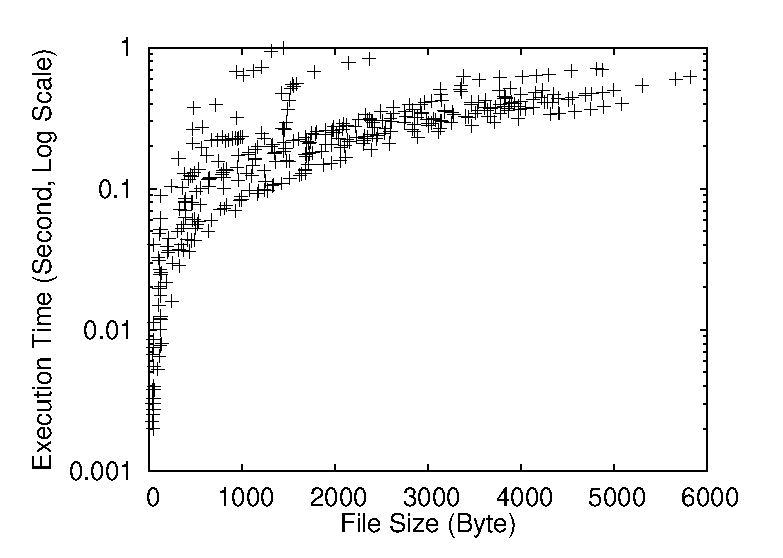
\epsfig{file=figure/endtoendTime.eps,width=1.05\columnwidth}
\caption{Wikification Time of Different File Sizes}
\label{fig:etime}
\end{subfigure}
\caption{Performance}
\end{figure}

%\begin{table}[h]
%\centering
%\begin{tabular}{|c|c|c|c|}
%\hline
%Sample Size & Cucerzan's & Kulkarni's & Cai's \\
%\hline
%Sample Size & Cucerzan's & Kulkarni's & Cai's \\
%\hline
%5000 & 81.22\% & 85.26\% & 90.82\% \\
%10000 & 81.01\% & 84.74\% & 91.42\% \\
%15000 & 81.01\% & 84.47\% & 90.42\% \\
%20000 & 81.22\% & 84.78\% & 91.62\% \\
%\hline
%\end{tabular}
%\caption{Precision on Different Data Set}
%\label{tab:precision}
%\end{table}
%
%\begin{table}[h]
%\centering
%\begin{tabular}{|c|c|c|c|}
%\hline
%Sample Size & Cucerzan's & Kulkarni's & Cai's \\
%\hline
%5000 & 76.85\% & 84.05\% & 90.82\% \\
%10000 & 76.65\% & 83.54\% & 91.42\% \\
%15000 & 76.65\% & 83.28\% & 90.42\% \\
%20000 & 76.85\% & 83.57\% & 91.62\% \\
%\hline
%\end{tabular}
%\caption{Recall on Different Data Set}
%\label{tab:recall}
%\end{table}
%
%\begin{table}[h]
%\centering
%\begin{tabular}{|c|c|c|c|}
%\hline
%Sample Size & Cucerzan's & Kulkarni's & Cai's \\
%\hline
%5000 & 78.97\% & 84.65\% & 90.82\% \\
%10000 & 78.77\% & 84.13\% & 91.42\% \\
%15000 & 78.77\% & 83.87\% & 90.42\% \\
%20000 & 78.97\% & 84.17\% & 91.62\% \\
%\hline
%\end{tabular}
%\caption{F1-measure on Different Data Set}
%\label{tab:f1}
%\end{table}






%%% Local Variables:
%%% mode: latex
%%% TeX-master: "paper"
%%% End:
